\documentclass[12pt]{report}

\usepackage[a4paper]{geometry}
\usepackage[utf8]{inputenc}
\usepackage[portuguese]{babel}
\usepackage{graphicx}

\newcommand\tab[1][0.5cm]{\hspace*{#1}}

\title{Projeto de Sistemas Operativos (MiEI) \\ 2017/2018}
\author{Alexandre Mendonça Pinho (a82441) \and Joel Filipe Esteves Gama (a82202) \and Tiago Martins Pinheiro (a82491)}
\date{\today}

\begin{document}
\maketitle

\tableofcontents

\chapter{Introdução}
\label{sec:introducao}

\tab Neste projeto é-nos proposto construir um sistema para processamento de notebooks, que misturam fragmentos de código, resultados da execução, e documentação. Estes notebooks tratam-se de ficheiros de texto que são modificados de modo a incluir os resultados da execução dos comandos neles embebidos.

\chapter{Descrição do projeto}
\label{sec:descricao}

 Para resolver o problema que nos foi apresentado começamos por fazer o parsing do ficheiro. O parsing excluí o output dos comandos (se presente) da escrita final e constroi o grafo de execução, cujos nodos correspondem a comandos a executar e cujas arestas são os redicionamentos dos outputs dos comandos. Se um nodo A do grafo tem uma aresta vinda de outro nodo B, isto significa que o output de B será redirecionado como o input de A. Como um nodo apenas pode conter uma origem do seu input, o grafo formado será um conjunto de árvores. A raiz de cada uma destas árvores recebe o seu output, por ordem de execução como o ficheiro de input sugere, do standard input. Em cada uma destas árvores, os processos são executados em paralelo, mas como em cada instante não é desejável estarem em execução dois processos que leem do standard input, o programa espera que o anterior dos dois termine ante de iniciar o seguinte.

 Para além de alimentar os outros processos com o seu input se necessário, o output dos comando é também escrito num FIFO reservado a ser lido pelo programa principal, para posteriormente ser escrito de volta para o notebook.

 Aquando da execução dos comandos, o seu output é primeiro redirecionado para um outro programa, um distribuidor, através de um pipe anónimo. O programa distribuidor recebe como argumentos os nomes dos ficheiros para os quais deve escrever o que lê no seu input. Serve assim para duplicar e distribuir o output de um processo para vários FIFOs.

 Depois da execução de todos os comandos, os seus outputs são incluidos no string (representado como uma lista ligada de blocos contendo cada um um buffer, para mais fácil introdução de novo conteúdo) que será escrito para ficheiro. É apenas no final que este string é escrito para ficheiro, permitindo ao utilizador cancelar o processamento do notebook a meio do programa sem alterar o ficheiro de input.

\chapter{Exemplo}

\label{sec:exemplo}

Ficheiro de input exemplo:

\begin{small}
\texttt{
\newline Listagem da diretoria atual
\newline \$ ls\newline
\newline O número de ficheiros na listagem
\newline \$ | wc -l\newline
\newline O nome do primeiro elemento
\newline \$ 2 | head -1\newline
\newline Aceitar input do utilizador
\newline \$ cat
}
\end{small}

\begin{figure}
    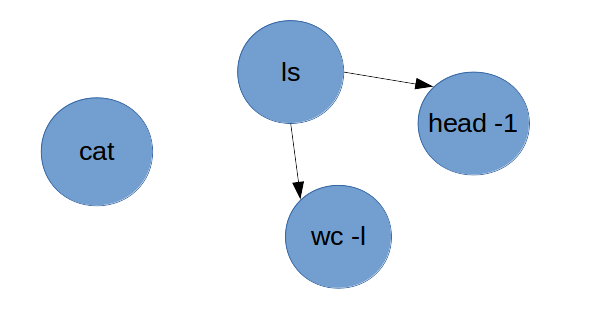
\includegraphics[width=\linewidth]{grafo_execucao_exemplo.png}
    \caption{Grafo de execução}
    \label{fig:grafo_execucao}
\end{figure}

\break
A figura \ref{fig:grafo_execucao} mostra a representação visual do grafo de execução contruido pelo parsing do ficheiro de input. O output do comando \texttt{ls} é redirecionado para o comando \texttt{wc -l}, que conta o número de linha da listagem da diretoria, e para o comando \texttt{head -1}, que imprime o nome do primeiro elemento da listagem. O grafo contém tambem o comando \texttt{cat}, que nos permite introduzir algum texto.

\begin{figure}
    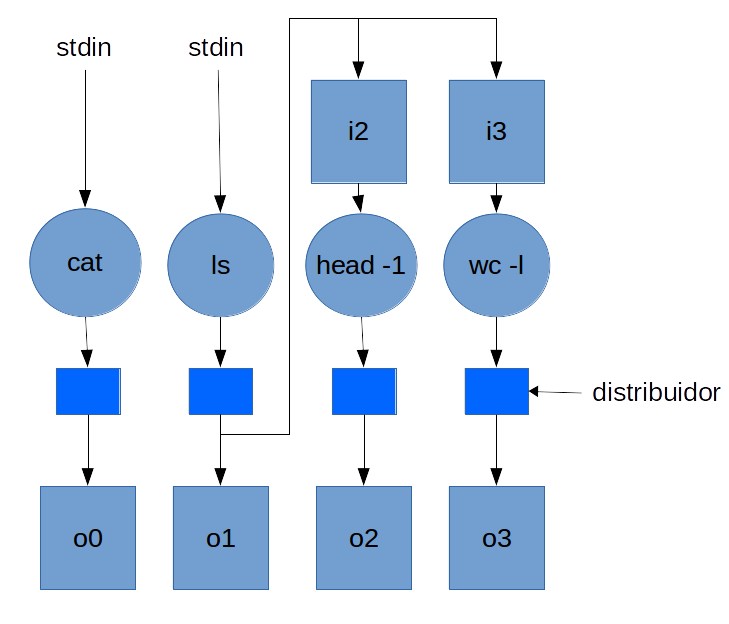
\includegraphics[width=\linewidth]{esquema_execucao_exemplo.png}
    \caption{Esquema de execução}
    \label{fig:esquema_execucao}
\end{figure}

 A figura \ref{fig:esquema_execucao} representa esquematicamente como o input e output dos processos são tratados. Para cada processo, é criado um FIFO em que vai ser escrito o seu output. Se esse processo aceitar o seu input de um outro processo aqui representado, como é o caso dos comandos \texttt{wc -l} e \texttt{head -1}, é também criado um FIFO onde será escrito o output do respetivo comando. Caso contrário (nos comandos \texttt{ls} e \texttt{cat}), o seu input é lido do standard input.

 O output de cada processo é redirecionado para o input do seu respetivo distribuidor através de um pipe anónimo. Este distribuidor foi inicializado com o nome do FIFO de output e, no caso dos processos cujo input é pedido por outros processos, também com os nomes dos FIFOs de input dos ditos processos.

\noindent Ficheiro de output resultante, ao introduzir pelo no teclado o string "Hello, world!\textbackslash n" (seguido da tecla ctrl-d para terminar o input):

\begin{small}
\fontsize{10}{12}\selectfont
\texttt{
\newline Listagem da diretoria atual
\newline \$ ls
\newline >>>
\newline distribuidor \newline distribuidor.c \newline i1 \newline i2
\newline include \newline lib \newline main.c \newline Makefile
\newline notebook \newline o0 \newline o1 \newline o2 \newline o3
\newline obj \newline README.md \newline relatorio \newline test
\newline <<<
\newline O número de ficheiros na listagem
\newline \$ | wc -l
\newline >>>
\newline 17
\newline <<<
\newline O nome do primeiro elemento
\newline \$ 2 | head -1
\newline >>>
\newline distribuidor
\newline <<<
\newline Aceitar input do utilizador
\newline \$ cat
\newline >>>
\newline Hello, world!
\newline <<<
\newline
}
\end{small}

\chapter{Conclusão}
\label{sec:conclusao}

\tab Foi-nos prosposto, como projeto de avaliação, conceber um sistema que fosse capaz de processar \textit{notebooks}, através da sua leitura e  interpretação. A implementação foi feita na linguagem de programação \textit{C}, utilizando os conceitos aprendidos durante as aulas práticas ao longo do semestre. 

Para os métodos de comunicação entre processos, escolhemos pipes anónimos para comunicar entre os processos e os distribuidores, e \textit{fifos} para comunicar entre os diferentes processos através dos distribuidores. Assim, a comunicação entre processos é tratada de forma simples pelos distribuidores.

\end{document}
